% Provenance (never printed): see sources/outline_sources.md (Year 2: viscosity, density and
% volatiles of magmas; magma ascent; dykes, sills and plutons; contact aureoles).
% Curves from figdata/bachelor-2/magma.py (GRD 2008 viscosity, DensityX density, Moore 1998
% solubility data, erf sill cooling, Stefan solidification); exercise and problem values in
% the Book 4 scratch calculators calc/ch05.py and calc/ch05pb.py.
\chapter{Los magmas y su emplazamiento}\label{ch:b2:magma-emplacement}

Un fundido basáltico a \qty{1200}{\celsius} fluye con una viscosidad de unos
\qty{70}{Pa.s}: espeso, pero se vierte. Un fundido riolítico seco a \qty{800}{\celsius}
tiene una viscosidad cercana a \qty{e11}{Pa.s}, y un bloque de él tardaría horas en combarse
de forma visible bajo su propio peso. Entre ambos hay diez órdenes de magnitud, más
que entre el agua y el basalto, y la mayor parte de la diferencia se debe a dos
cosas: la sílice, que enlaza el fundido en una red, y la temperatura,
que es varios cientos de grados más baja en los \omterm{def:b2:magma-emplacement:magma}{magmas} silícicos. Unos pocos por ciento de
agua disuelta, que un \omterm{def:b2:magma-emplacement:magma}{magma} riolítico puede contener en profundidad, reducen su viscosidad
en un factor \num{e5}, y el \omterm{def:b2:magma-emplacement:magma}{magma} vuelve a perderlos a medida que sube y el
agua sale en forma de burbujas. Estos números deciden si un \omterm{def:b2:magma-emplacement:magma}{magma} llega a la
superficie con calma, explota o se congela a kilómetros de profundidad como \omterm{def:b2:magma-emplacement:bodies}{dique}, \omterm{def:b2:magma-emplacement:bodies}{filón capa} o
\omterm{def:b2:magma-emplacement:bodies}{plutón}. Este capítulo trata el \omterm{def:b2:magma-emplacement:magma}{magma} como un material: su densidad, su viscosidad y sus
volátiles, la física de su ascenso por grietas y en forma de masas, las formas que
adopta cuando se detiene, y el calor que cede a las rocas que lo rodean.
% ledger: grd08:model, grd08:range, moore98:melts

\begin{recall}
\textbf{Flujo viscoso} (volumen de segundo año de los libros de física): en un fluido newtoniano de
viscosidad $\eta$ la tensión de cizalla es $\eta$ por el gradiente de velocidad; entre
dos paredes paralelas un gradiente de presión impone un perfil parabólico (de Poiseuille
plano); una esfera que se mueve despacio en un fluido viscoso sufre el arrastre de Stokes
$6\pi\eta a v$. \textbf{Conducción del calor} (mismo volumen): la temperatura obedece a
$\partial T/\partial t = \kappa\,\partial^2T/\partial x^2$, con difusividad $\kappa = k/(\rho
c)$, y un escalón de temperatura se extiende como una función error sobre una distancia del
orden de $\sqrt{\kappa t}$. \textbf{Flotabilidad} (volumen de primer año de los libros de física): un cuerpo
sumergido en un fluido más denso sufre una fuerza neta hacia arriba igual al peso del fluido
desalojado menos el suyo propio. \textbf{Equilibrio químico} (libros de química): en el
equilibrio las actividades de productos y reactivos cumplen la ley de acción de
masas con una constante $K$ que depende de la temperatura. Del volumen de primer año
de esta serie: la presión litostática $p = \rho g z$ y la geoterma; de los
volúmenes escolares: rocas máficas y félsicas, fenocristales y texturas porfídicas.
\end{recall}

\section{Qué es un magma}

\begin{definition}[Magma]\label{def:b2:magma-emplacement:magma}
Un \emph{magma}\index{magma} es roca fundida o parcialmente fundida bajo la superficie: un
\emph{fundido silicatado}\index{fundido silicatado}, el líquido formado sobre todo por silicio,
oxígeno y cationes metálicos, junto con los cristales y las burbujas de gas que lleve.
Una \emph{papilla cristalina}\index{papilla cristalina} es un magma tan rico en cristales que estos
se tocan y forman un armazón: no puede fluir como un líquido, y su fundido solo puede
moverse por los poros entre los cristales.
\end{definition}

La composición del fundido se da, como la de las rocas, en porcentaje en masa de
óxidos. Tres fundidos sirven de referencia a lo largo del capítulo, todos ellos
estudiados en el laboratorio: un basalto toleítico dragado en una dorsal oceánica
(cerca de un \qty{51}{\percent} de SiO$_2$, un \qty{12}{\percent} de óxido de hierro y un \qty{7}{\percent} de
MgO), una andesita (\qty{63}{\percent} de SiO$_2$) y una riolita (\qty{78}{\percent} de
SiO$_2$, \qty{8}{\percent} de Na$_2$O $+$ K$_2$O y casi nada de hierro ni de magnesio).
Sus temperaturas de erupción difieren tanto como sus composiciones: los \omterm{def:b2:magma-emplacement:magma}{magmas}
basálticos entran en erupción de \qtyrange{1000}{1200}{\celsius} (la lava que corre por un tubo del
Kilauea se ha medido cerca de \qty{1200}{\celsius}), los andesíticos de
\qtyrange{800}{1000}{\celsius} y los riolíticos de \qtyrange{650}{800}{\celsius}.
Un \omterm{def:b2:magma-emplacement:magma}{magma} riolítico es más frío porque es el residuo de una larga cristalización
o el primer fundido de rocas corticales, dos procesos que ocurren a baja temperatura
(\cref{ch:b2:magmatic-differentiation}).
% ledger: moore98:melts, tulane:magma-types, earle:kilauea-lava

El contenido en cristales decide si un \omterm{def:b2:magma-emplacement:magma}{magma} fluye. Los estudios de campo y geocronológicos
de grandes cuerpos graníticos concluyen que el flujo magmático en masa requiere una fracción
de fundido de al menos un \qtyrange{30}{50}{\percent} en volumen; por debajo, los
cristales quedan soldados a sus vecinos y el material se deforma como un sólido con
poros llenos de fundido. Se cree que buena parte del \omterm{def:b2:magma-emplacement:magma}{magma} almacenado en la corteza está en
ese estado, como una papilla que vuelve a ser móvil cuando se le añade \omterm{def:b2:magma-emplacement:magma}{magma} caliente desde
abajo.
% ledger: glazner04:tuolumne

\section{Densidad y viscosidad}

\subsection{La densidad de un fundido}

Un \omterm{def:b2:magma-emplacement:magma}{fundido silicatado} no tiene red cristalina, pero su volumen puede construirse igualmente a partir de
sus componentes. Los experimentos con muchos fundidos muestran que cada óxido aporta un
volumen casi fijo por mol, su volumen molar parcial, que cambia lenta y
linealmente con la temperatura y la presión; el volumen del fundido es la suma de
estas contribuciones. La tabla siguiente da los valores usados en este capítulo.

\begin{table}[ht]
\centering\small
\begin{tabular}{lrrr}
\hline
Óxido & $\bar V_i$ (\unit{cm^3/mol}) & $\partial\bar V_i/\partial T$ (\num{e-3}\,\unit{cm^3/(mol.K)}) & $\partial\bar V_i/\partial p$ (\num{e-4}\,\unit{cm^3/(mol.bar)}) \\
\hline
SiO$_2$  & 26.86 & 0     & $-1.89$ \\
Al$_2$O$_3$ & 37.42 & 2.62 & $-2.26$ \\
FeO      & 12.68 & 3.69  & $-0.45$ \\
MgO      & 12.02 & 3.27  & $0.27$ \\
CaO      & 16.90 & 3.74  & $0.34$ \\
Na$_2$O  & 29.65 & 7.68  & $-2.40$ \\
K$_2$O   & 47.28 & 12.08 & $-6.75$ \\
H$_2$O   & 22.9  & 9.5   & $-3.20$ \\
\hline
\end{tabular}
\caption{Volúmenes molares parciales de los componentes óxidos en los \omterm{def:b2:magma-emplacement:magma}{fundidos silicatados} a
\qty{1}{bar}, con sus derivadas respecto a la temperatura y la presión. Temperatura de
referencia \qty{1773}{K} (FeO \qty{1723}{K}, H$_2$O \qty{1273}{K}). Datos:
compilación del programa DensityX (Iacovino y Till, 2019).}
\label{tab:b2:magma-emplacement:volumes}
\end{table}
% ledger: densityx:volumes

\begin{proposition}[Densidad de un fundido silicatado]\label{prop:b2:magma-emplacement:density}
Contenga un fundido componentes óxidos $i$ con fracciones molares $X_i$, masas molares
$M_i$ y volúmenes molares parciales $\bar V_i(T, p) = \bar V_i^{\circ} + (\partial\bar
V_i/\partial T)(T - T_{\mathrm{ref}}) + (\partial\bar V_i/\partial p)(p - p_{\mathrm{ref}})$.
Si los componentes se mezclan idealmente en volumen,
\[
\rho = \frac{\sum_i X_i M_i}{\sum_i X_i \bar V_i(T,p)}.
\]
\end{proposition}

\begin{proof}
Un mol de fundido contiene $X_i$ moles del componente $i$, de masa $X_iM_i$. La mezcla
ideal en volumen significa que cada mol del componente $i$ añade el volumen $\bar V_i$
sean cuales sean los demás, de modo que el mol de fundido ocupa $\sum_i X_i\bar V_i$. La
densidad es el cociente de ambos.
\end{proof}

El agua tiene una masa molar de solo \qty{18}{g/mol} pero un volumen molar parcial de
\qty{22.9}{cm^3/mol}, cercano al de la sílice: reduce mucho la densidad de un
fundido. Aplicada a los tres fundidos de referencia, la proposición da
\qty{2730}{kg/m^3} para el basalto a \qty{1200}{\celsius}, \qty{2480}{kg/m^3} para
la andesita a \qty{1000}{\celsius} y \qty{2340}{kg/m^3} para la riolita seca
a \qty{850}{\celsius}; un uno por ciento de agua disuelta resta unos
\qty{70}{kg/m^3} al basalto, tanto como varios cientos de grados de calentamiento.
Un fundido basáltico es por tanto más ligero que la peridotita del manto de la que procede
(unos \qty{3380}{kg/m^3} bajo la corteza en el modelo terrestre de referencia) y algo
más ligero que la corteza inferior de ese modelo (\qty{2900}{kg/m^3}), mientras que un
fundido riolítico es más ligero incluso que su corteza superior (\qty{2600}{kg/m^3}). Esta diferencia impulsa los \omterm{def:b2:magma-emplacement:magma}{magmas}
hacia arriba.
% ledger: densityx:volumes, densityx:water, data:prem

\subsection{Viscosidad}

La viscosidad de un \omterm{def:b2:magma-emplacement:magma}{fundido silicatado} la fija la red de tetraedros SiO$_4$
enlazados por oxígenos compartidos: para fluir, el fundido debe romper y rehacer
enlaces silicio--oxígeno. La sílice y la alúmina construyen la red; los cationes de
magnesio, hierro, calcio y los alcalinos la rompen, y también el agua, que
convierte los oxígenos puente en grupos hidroxilo. Las medidas de laboratorio en fundidos
naturales abarcan más de quince órdenes de magnitud, de \qty{0.1}{Pa.s} a
\qty{e14}{Pa.s}, y no siguen una ley de Arrhenius sencilla: la viscosidad
crece más deprisa que una exponencial en $1/T$ a medida que el fundido se enfría hacia su
transición vítrea.
% ledger: grd08:range

\begin{proposition}[Ley de Vogel--Fulcher--Tammann]\label{prop:b2:magma-emplacement:vft}
La viscosidad de un \omterm{def:b2:magma-emplacement:magma}{fundido silicatado} de composición fija sigue, con un margen de unas pocas
décimas de unidad logarítmica,
\[
\log_{10}\eta = A + \frac{B}{T - C},
\]
con $\eta$ en pascales segundo y $T$ en kelvin. Para los fundidos naturales $A$ es cercano
a $-4.55$ sea cual sea la composición; $B$ y $C$ (en kelvin) son combinaciones
lineales de los porcentajes molares de los óxidos, con algunos productos de ellos,
ajustadas a unas \num{1800} medidas.
\end{proposition}
\admitted
% ledger: grd08:model, grd08:range

La figura siguiente muestra la ley para los tres fundidos de referencia y para la
riolita con agua disuelta. A \qty{1200}{\celsius} el basalto tiene
$\eta \approx \qty{70}{Pa.s}$; la andesita a \qty{1000}{\celsius} tiene unos
\qty{e6}{Pa.s}; la riolita seca a \qty{800}{\celsius}, unos $10^{10.9}$\,\unit{Pa.s}.
Un cuatro por ciento de agua baja esa misma riolita a $10^{5.5}$\,\unit{Pa.s}, y un seis
por ciento a $10^{4.6}$\,\unit{Pa.s}. Una ecuación independiente ajustada solo a fundidos
graníticos hidratados da los mismos valores con un margen de media unidad logarítmica
(\cref{exo:b2:magma-emplacement:1}). El efecto del agua es máximo a baja temperatura, donde unas pocas
décimas de por ciento cambian la viscosidad en órdenes de magnitud.
% ledger: grd08:model, hd96:model, moore98:melts

\begin{omfigure}
\centering
\begin{tikzpicture}
\begin{axis}[omrecord, width=0.86\linewidth, height=6.4cm,
  xmin=600, xmax=1400, ymin=0, ymax=15,
  xlabel={temperatura (\unit{\celsius})}, ylabel={$\log_{10}\eta$ (\unit{Pa.s})},
  legend pos=north east, legend style={font=\scriptsize},
  tick label style={font=\scriptsize}, label style={font=\small}]
\addplot[very thick, black, restrict x to domain=1000:1400] table[x=T_C, y=basalt] {figdata/out/bachelor-2-magma-visc.dat};
\addlegendentry{basalto, seco}
\addplot[very thick, brown, restrict x to domain=800:1300] table[x=T_C, y=andesite] {figdata/out/bachelor-2-magma-visc.dat};
\addlegendentry{andesita, seca}
\addplot[very thick, red!70!black, restrict x to domain=650:1100] table[x=T_C, y=rhyolite] {figdata/out/bachelor-2-magma-visc.dat};
\addlegendentry{riolita, seca}
\addplot[thick, red!70!black, dashed, restrict x to domain=650:1000] table[x=T_C, y=rhy2] {figdata/out/bachelor-2-magma-visc.dat};
\addlegendentry{riolita, 2 \% de H$_2$O}
\addplot[thick, red!70!black, densely dotted, restrict x to domain=650:1000] table[x=T_C, y=rhy4] {figdata/out/bachelor-2-magma-visc.dat};
\addlegendentry{riolita, 4 \% de H$_2$O}
\addplot[thick, red!70!black, dashdotted, restrict x to domain=650:1000] table[x=T_C, y=rhy6] {figdata/out/bachelor-2-magma-visc.dat};
\addlegendentry{riolita, 6 \% de H$_2$O}
\end{axis}
\end{tikzpicture}
\par\smallskip{\small Viscosidad de los \omterm{def:b2:magma-emplacement:magma}{fundidos silicatados} frente a la temperatura, según la
ley de Vogel--Fulcher--Tammann con los parámetros dependientes de la composición de
Giordano, Russell y Dingwell (2008). Basalto: una toleíta de dorsal oceánica;
andesita y riolita: fundidos de referencia de laboratorio (Moore y colaboradores, 1998). Cada
curva se traza en el intervalo de temperaturas en que un \omterm{def:b2:magma-emplacement:magma}{magma} así puede estar fundido.}
\end{omfigure}
% ledger: grd08:model, moore98:melts

Los cristales hacen el \omterm{def:b2:magma-emplacement:magma}{magma} aún más rígido. Una suspensión de partículas rígidas resiste
la cizalla más que su líquido solo, porque el líquido debe fluir alrededor de las
partículas, y cuando las partículas están tan apretadas que se tocan se traban en un
armazón.

\begin{proposition}[Relación de Einstein--Roscoe]\label{prop:b2:magma-emplacement:roscoe}
Una suspensión de una fracción de volumen $\phi$ de esferas rígidas en un líquido newtoniano
de viscosidad $\eta_{\ell}$ tiene la viscosidad
\[
\eta = \eta_{\ell}\,(1 - R\phi)^{-2.5}, \qquad R = 1/\phi_m \approx 1.35,
\]
donde $\phi_m$ es la fracción de empaquetamiento máxima, a la que la suspensión se bloquea. Para
$\phi$ pequeña se reduce a la de Einstein, $\eta = \eta_{\ell}(1 + 2.5\phi)$.
\end{proposition}
\admitted
% ledger: kolz22:einstein-roscoe

Un veinte por ciento de cristales duplica la viscosidad, un cuarenta por ciento la multiplica por
siete y un sesenta por ciento por más de sesenta (\cref{exo:b2:magma-emplacement:5}); en los \omterm{def:b2:magma-emplacement:magma}{magmas} reales, donde los
cristales son alargados y de muchos tamaños, el bloqueo llega antes, hacia un
\qtyrange{50}{70}{\percent} de cristales en que los datos de campo sitúan el
final del flujo en masa.

\section{Volátiles}

\begin{definition}[Volátiles magmáticos]\label{def:b2:magma-emplacement:volatiles}
Un \emph{volátil magmático}\index{volátil magmático} es un componente de un \omterm{def:b2:magma-emplacement:magma}{magma} que
está disuelto en el fundido en profundidad y forma una fase gaseosa separada a baja
presión: sobre todo agua, luego dióxido de carbono, luego especies de azufre. La \emph{exsolución
de volátiles}\index{exsolución de volátiles} es la separación de un volátil del
fundido en burbujas de gas. La \emph{presión de saturación en
volátiles}\index{presión de saturación en volátiles} de un fundido es la presión por debajo de la cual
sus volátiles disueltos superan su solubilidad, de modo que debe formarse una fase gaseosa.
\end{definition}

Los \omterm{def:b2:magma-emplacement:magma}{magmas} máficos llevan típicamente un \qtyrange{1}{3}{\percent} de volátiles en masa,
los intermedios un \qtyrange{3}{4}{\percent} y los félsicos un
\qtyrange{4}{7}{\percent}, y la exsolución de un \qtyrange{4}{6}{\percent} de
agua impulsa la mayoría de las erupciones explosivas. Cuánta agua puede contener un fundido depende
ante todo de la presión. La figura siguiente muestra medidas en fundidos basálticos y
riolíticos mantenidos a una presión de agua conocida hasta la saturación, templados luego
a vidrio y analizados: la solubilidad crece deprisa a baja presión y más
despacio a alta presión.
% ledger: earle:volatiles, moore98:arc-water, moore98:h2o

\begin{proposition}[Ley de la raíz cuadrada para el agua]\label{prop:b2:magma-emplacement:sqrt}
Supóngase que el agua se disuelve en un \omterm{def:b2:magma-emplacement:magma}{fundido silicatado} sobre todo como grupos hidroxilo, mediante
la reacción $\mathrm{H_2O\,(gas)} + \mathrm{O^{2-}\,(melt)} \rightleftharpoons
2\,\mathrm{OH^-\,(melt)}$, con el oxígeno del fundido en gran exceso. Entonces, con
contenidos de agua bajos, el agua disuelta es proporcional a la raíz cuadrada de
la presión de agua: $w \approx s\sqrt{p}$, con $s$ una constante del fundido y de la
temperatura.
\end{proposition}

\begin{proof}
La ley de acción de masas da $x_{\mathrm{OH}}^2 = K\,x_{\mathrm{O}}\,f$, donde $f$ es
la fugacidad del agua (cercana a su presión a presiones moderadas) y las $x$
son fracciones molares. El oxígeno del fundido está en gran exceso, de modo que
$x_{\mathrm{O}}$ permanece casi constante, y $x_{\mathrm{OH}} = \sqrt{Kx_{\mathrm{O}}}\,
\sqrt f$. Cada molécula de agua disuelta forma dos hidroxilos, de modo que el agua
disuelta es $x_{\mathrm{OH}}/2$, proporcional a $\sqrt f$. Con contenidos mayores parte
del agua se disuelve como moléculas, en proporción a la propia $f$, y la
solubilidad crece más deprisa que la raíz cuadrada (\cref{exo:b2:magma-emplacement:10}).
\end{proof}

Ajustada por mínimos cuadrados a las medidas, $w = s\sqrt p$ da
$s = 0.34$ por ciento en masa por $\sqrt{\unit{MPa}}$ para los basaltos y
$s = 0.44$ para las riolitas; todas las medidas quedan a menos de un uno por ciento de
agua de su curva. La presión de saturación de un fundido con un $w$ por ciento
de agua es entonces $p_s = (w/s)^2$: \qty{129}{MPa} para una riolita con un
\qty{5}{\percent} de agua, a unos \qty{5}{km} de profundidad en la corteza, pero solo
\qty{2}{MPa} para un basalto con un \qty{0.5}{\percent}, a cien metros o menos.
% ledger: moore98:h2o

\begin{omfigure}
\centering
\begin{tikzpicture}
\begin{axis}[omrecord, width=0.8\linewidth, height=6cm,
  xmin=0, xmax=300, ymin=0, ymax=9,
  xlabel={presión de agua (\unit{MPa})}, ylabel={H$_2$O disuelta (\% en masa)},
  legend pos=south east, legend style={font=\scriptsize},
  tick label style={font=\scriptsize}, label style={font=\small}]
\addplot[very thick, red!70!black] table[x=P_MPa, y=rhyolite] {figdata/out/bachelor-2-magma-solub-fit.dat};
\addlegendentry{riolita, $0.44\sqrt p$}
\addplot[only marks, mark=*, mark size=2pt, red!70!black] table[x=P_MPa, y=w] {figdata/out/bachelor-2-magma-solub-rhyolite-data.dat};
\addlegendentry{riolita, medida}
\addplot[very thick, black] table[x=P_MPa, y=basalt] {figdata/out/bachelor-2-magma-solub-fit.dat};
\addlegendentry{basalto, $0.34\sqrt p$}
\addplot[only marks, mark=square*, mark size=2pt, black] table[x=P_MPa, y=w] {figdata/out/bachelor-2-magma-solub-basalt-data.dat};
\addlegendentry{basalto, medida}
\end{axis}
\end{tikzpicture}
\par\smallskip{\small Solubilidad del agua en fundidos basálticos y riolíticos de
\qtyrange{800}{1200}{\celsius} frente a la presión de agua: medidas compiladas
por Moore y colaboradores (1998), y leyes de raíz cuadrada ajustadas por mínimos cuadrados. A
\qty{100}{MPa}, a unos \qty{4}{km} de profundidad en la corteza, una riolita puede contener un
\qty{4.4}{\percent} de agua, y un basalto un \qty{3.4}{\percent}.}
\end{omfigure}
% ledger: moore98:h2o

El dióxido de carbono es mucho menos soluble que el agua. Se disuelve como moléculas en
las riolitas y como grupos carbonato en los basaltos, más en los fundidos alcalinos que en las
toleítas, y su solubilidad también crece con la presión. Un \omterm{def:b2:magma-emplacement:magma}{magma} que lleva ambos
gases empieza por tanto a exsolverlos en profundidad, con un gas muy rico en CO$_2$, y el
gas se enriquece en agua a medida que el \omterm{def:b2:magma-emplacement:magma}{magma} sube. Los basaltos emitidos en el fondo
oceánico profundo contienen vesículas de más de un \qty{95}{\percent} de CO$_2$, lo que exigió
la saturación en CO$_2$ incluso bajo \qty{5}{km} de agua. Las estimaciones del contenido inicial en
CO$_2$ de los basaltos parentales del Kilauea van de \qtyrange{0.2}{0.6}{\percent},
y las inclusiones de fundido atrapadas en sus cristales de olivino registran presiones de
saturación de hasta \qty{500}{MPa}.
% ledger: lowenstern01:co2, lowenstern01:basalts

El gas exsuelto ocupa un gran volumen. Un uno por ciento de agua en un \omterm{def:b2:magma-emplacement:magma}{magma} a
\qty{900}{\celsius} ocupa, como gas ideal, cerca del \qty{12}{\percent} del
volumen a \qty{100}{MPa}, el \qty{57}{\percent} a \qty{10}{MPa} y más del
\qty{99}{\percent} a la presión atmosférica (\cref{exo:b2:magma-emplacement:7}). Las burbujas bajan
aún más la densidad del \omterm{def:b2:magma-emplacement:magma}{magma} y lo impulsan hacia arriba más deprisa; en un \omterm{def:b2:magma-emplacement:magma}{magma} viscoso
no pueden escapar, y el \cref{ch:b2:eruptive-styles} muestra cómo lo fragmentan.

\section{El ascenso}

Un cuerpo de \omterm{def:b2:magma-emplacement:magma}{magma} menos denso que su entorno sufre una fuerza de flotabilidad de
$\Delta\rho\,g$ por unidad de volumen, donde $\Delta\rho$ es la diferencia de densidad.
Puede subir de dos maneras: por una grieta que abre por delante de sí, o como una masa
caliente y blanda que aparta la roca circundante.

\subsection{Los diques}

En profundidad la roca está sometida a una gran presión litostática, pero una grieta llena
de \omterm{def:b2:magma-emplacement:magma}{magma} a una presión algo mayor que el esfuerzo principal mínimo puede
abrirse y alargarse por su extremo. El \omterm{def:b2:magma-emplacement:magma}{magma} llena la grieta a medida que crece, y el resultado
es una lámina delgada de \omterm{def:b2:magma-emplacement:magma}{magma}, de metros de anchura y kilómetros de longitud, que se abre camino
hacia arriba: un \omterm{def:b2:magma-emplacement:bodies}{dique} en formación. El \omterm{def:b2:magma-emplacement:magma}{magma} fluye entonces entre dos paredes
casi paralelas.

\begin{proposition}[Flujo del magma en un dique]\label{prop:b2:magma-emplacement:poiseuille}
Un \omterm{def:b2:magma-emplacement:magma}{magma} newtoniano de viscosidad $\eta$ impulsado hacia arriba por un gradiente de presión $G$
(en el flujo por flotabilidad, $G = \Delta\rho\,g$) entre dos paredes paralelas separadas una distancia $w$
fluye con la velocidad media
\[
\bar u = \frac{G w^2}{12\,\eta},
\]
y el caudal volumétrico por unidad de longitud de \omterm{def:b2:magma-emplacement:bodies}{dique} es $q = \bar u w = G w^3/(12\eta)$.
\end{proposition}

\begin{proof}
En un flujo laminar estacionario el perfil de velocidad a través del \omterm{def:b2:magma-emplacement:bodies}{dique} es la parábola
de Poiseuille plana $u(x) = \frac{G}{2\eta}\left(\frac{w^2}{4} - x^2\right)$, para
$-w/2 \le x \le w/2$, que se anula en ambas paredes. Su media es
$\bar u = \frac1w\int_{-w/2}^{w/2}u\,dx = \frac{G}{2\eta}\left(\frac{w^2}{4} -
\frac{w^2}{12}\right) = \frac{Gw^2}{12\eta}$.
\end{proof}

El cubo de la anchura hace los \omterm{def:b2:magma-emplacement:bodies}{diques} anchos mucho más eficaces que los estrechos. Un
basalto de \qty{100}{Pa.s} en un \omterm{def:b2:magma-emplacement:bodies}{dique} de \qty{1}{m} de anchura, con $\Delta\rho =
\qty{300}{kg/m^3}$, sube a unos \qty{2.5}{m/s} y atraviesa \qty{10}{km} de
corteza en una hora; una riolita de \qty{e6}{Pa.s} en el mismo \omterm{def:b2:magma-emplacement:bodies}{dique} tardaría más
de un año, y se congelaría por el camino, de modo que los \omterm{def:b2:magma-emplacement:magma}{magmas} silícicos necesitan \omterm{def:b2:magma-emplacement:bodies}{diques}
mucho más anchos (\cref{exo:b2:magma-emplacement:6}). El número de Reynolds $\rho\bar u w/\eta$ de estos flujos
es lo bastante pequeño para que sigan siendo laminares. Las velocidades de ascenso estimadas para los \omterm{def:b2:magma-emplacement:magma}{magmas}
durante las erupciones separan las erupciones efusivas, por debajo de unos \qty{0.1}{m/s}, de las
explosivas, por encima, con un intervalo de transición de \qtyrange{0.005}{0.25}{m/s}
en el que se dan ambos estilos; las kimberlitas, que proceden de
profundidades de más de \qty{150}{km}, se han estimado en \qtyrange{0.1}{30}{m/s}, y
un estudio de difusión de una de ellas da \qtyrange{0.02}{0.23}{m/s} de media en
los últimos \qtyrange{80}{110}{km}, un viaje de \numrange{5}{74} días.
% ledger: cassidy18:ascent, casetta23:kimberlite

\subsection{Los diapiros}

\begin{definition}[Diapiro, nivel de flotabilidad neutra, stoping]\label{def:b2:magma-emplacement:ascent}
Un \emph{diapiro}\index{diapiro} es un cuerpo de material flotante, \omterm{def:b2:magma-emplacement:magma}{magma} o roca parcialmente
fundida, que sube a través de su entorno apartándolo al fluir. El
\emph{nivel de flotabilidad neutra}\index{nivel de flotabilidad neutra} de un \omterm{def:b2:magma-emplacement:magma}{magma} es la
profundidad a la que su densidad es igual a la de la roca circundante: por debajo, el
\omterm{def:b2:magma-emplacement:magma}{magma} flota; por encima, es más denso que su entorno. El \emph{stoping
magmático}\index{stoping magmático} es el desprendimiento de bloques de la roca de las paredes o del
techo, que se hunden en el \omterm{def:b2:magma-emplacement:magma}{magma}; los bloques que quedan englobados en la roca
solidificada son xenolitos.
\end{definition}
% ledger: earle:intrusive-bodies

\begin{proposition}[Ascenso de Stokes]\label{prop:b2:magma-emplacement:stokes}
Una esfera de radio $a$ y déficit de densidad $\Delta\rho$ que sube despacio a través de un
medio newtoniano de viscosidad $\eta$ alcanza la velocidad terminal
\[
v = \frac{2\,\Delta\rho\,g\,a^2}{9\,\eta}
\]
si es rígida, y $1.5$ veces esta si es un fluido de viscosidad despreciable.
\end{proposition}
\admitted

La roca que rodea un \omterm{def:b2:magma-emplacement:ascent}{diapiro} no es un fluido de \qty{100}{Pa.s} sino un sólido caliente,
cuya viscosidad es muchos órdenes de magnitud mayor que la de cualquier fundido: en la
corteza, una esfera de \omterm{def:b2:magma-emplacement:magma}{magma} de un kilómetro de diámetro sube solo milímetros al año, y
pierde su calor mucho antes de haber subido lejos (\cref{exo:b2:magma-emplacement:9}). Los \omterm{def:b2:magma-emplacement:ascent}{diapiros}
funcionan donde el entorno es caliente y blando, en el manto y en las raíces
profundas de las cordilleras, y donde el material flotante es una masa parcialmente fundida
de kilómetros de diámetro; la corteza somera la atraviesan los \omterm{def:b2:magma-emplacement:bodies}{diques}.

\section{El emplazamiento}

La mayor parte del \omterm{def:b2:magma-emplacement:magma}{magma} nunca llega a la superficie. Se detiene donde deja de flotar,
o donde lo bloquea una capa más resistente, y se extiende en un cuerpo cuya forma
registra cómo se hizo sitio.

\begin{definition}[Cuerpos intrusivos]\label{def:b2:magma-emplacement:bodies}
Un \emph{plutón}\index{plutón} es cualquier cuerpo de \omterm{def:b2:magma-emplacement:magma}{magma} que se solidificó dentro de la
corteza. Un \emph{dique}\index{dique} es un plutón laminar que corta la
estratificación de su roca encajante (o cualquier lámina si el encajante no está estratificado); un
\emph{filón capa}\index{filón capa} es un plutón laminar paralelo a la estratificación. Un
\emph{lacolito}\index{lacolito} es un filón capa que ha engrosado levantando las
capas suprayacentes en forma de domo. Un \emph{batolito}\index{batolito} es un gran plutón,
o un conjunto de plutones, con una superficie aflorante de más de \qty{100}{km^2}.
\end{definition}
% ledger: earle:intrusive-bodies

\begin{omfigure}
\centering
\begin{tikzpicture}[x=1cm, y=1cm, font=\scriptsize]
% layered host
\fill[lith sandstone] (0,4.4) rectangle (12,5.4);
\fill[lith sandstone] (0,4.4) rectangle (12,5.4);
\fill[lith shale] (0,3.3) -- (0,4.4) -- (5.2,4.4) .. controls (5.7,4.95) and (7.0,4.95) .. (7.7,4.4)
  -- (12,4.4) -- (12,3.3) -- cycle;
\draw[thin] (0,4.4) -- (5.2,4.4) .. controls (5.7,4.95) and (7.0,4.95) .. (7.7,4.4) -- (12,4.4);
\fill[lith limestone] (0,2.2) rectangle (12,3.3);
\fill[lith sandstone] (0,0) rectangle (12,2.2);
\draw[thick] (0,0) rectangle (12,5.4);
% batholith at the bottom right
\fill[lith granite] (6.8,0) .. controls (7.2,1.6) and (8.4,2.2) .. (9.6,1.9)
  .. controls (10.6,1.7) and (11.2,1.3) .. (12,1.6) -- (12,0) -- cycle;
\draw[thick] (6.8,0) .. controls (7.2,1.6) and (8.4,2.2) .. (9.6,1.9)
  .. controls (10.6,1.7) and (11.2,1.3) .. (12,1.6);
% aureole around the batholith
\draw[densely dashed, orange!80!black, thick] (6.2,0) .. controls (6.6,2.2) and (8.4,2.8) .. (9.6,2.5)
  .. controls (10.6,2.3) and (11.3,2.0) .. (12,2.2);
% stoped blocks
\fill[lith limestone, draw=black] (8.4,1.0) rectangle (8.8,1.3);
\fill[lith sandstone, draw=black] (10.1,0.7) -- (10.5,0.8) -- (10.4,1.1) -- (10.0,1.0) -- cycle;
% feeder dyke from the bottom left, vertical
\fill[lith basalt] (2.0,0) rectangle (2.35,3.3);
\draw (2.0,0) -- (2.0,3.3) (2.35,0) -- (2.35,3.3);
% sill along shale/limestone contact
\fill[lith basalt] (2.0,3.15) rectangle (5.4,3.45);
\draw (2.0,3.15) -- (5.4,3.15) (2.35,3.45) -- (5.4,3.45);
% laccolith: lens pushing up the shale
\fill[lith basalt] (5.4,3.15) .. controls (5.6,3.95) and (6.6,4.05) .. (7.0,3.9)
  .. controls (7.3,3.8) and (7.4,3.4) .. (7.6,3.15) -- cycle;
\draw (5.4,3.45) .. controls (5.6,3.95) and (6.6,4.05) .. (7.0,3.9)
  .. controls (7.3,3.8) and (7.4,3.4) .. (7.6,3.15) -- (5.4,3.15);
% inclined dyke cutting to the surface from the laccolith
\fill[lith basalt] (6.6,3.95) -- (6.9,3.95) -- (7.6,5.4) -- (7.3,5.4) -- cycle;
% labels
\node[fill=white, fill opacity=0.8, text opacity=1, inner sep=1pt] at (1.2,1.4) {dique};
\draw (1.6,1.4) -- (2.0,1.4);
\node[fill=white, fill opacity=0.8, text opacity=1, inner sep=1pt] at (3.6,2.7) {filón capa};
\draw (3.6,2.85) -- (3.6,3.15);
\node[fill=white, fill opacity=0.8, text opacity=1, inner sep=1pt] at (6.2,4.75) {lacolito};
\draw (6.2,4.6) -- (6.3,3.95);
\node[fill=white, fill opacity=0.8, text opacity=1, inner sep=1pt] at (9.6,0.5) {batolito};
\node[fill=white, fill opacity=0.8, text opacity=1, inner sep=1pt, align=center] at (10.6,3.0) {aureola\\de contacto};
\draw (10.6,2.7) -- (10.8,2.3);
\node[fill=white, fill opacity=0.8, text opacity=1, inner sep=1pt, align=left] at (5.0,1.0) {bloques\\desprendidos};
\draw (5.6,1.0) -- (8.35,1.15);
\end{tikzpicture}
\par\smallskip{\small Formas de los cuerpos intrusivos en un encajante estratificado (esquema, sin
escala): un \omterm{def:b2:magma-emplacement:bodies}{dique} alimentador que corta las capas, un \omterm{def:b2:magma-emplacement:bodies}{filón capa} a lo largo de un plano de estratificación, un
\omterm{def:b2:magma-emplacement:bodies}{lacolito} que abomba las capas que tiene encima, un \omterm{def:b2:magma-emplacement:bodies}{dique} que corta hasta la superficie, y un
\omterm{def:b2:magma-emplacement:bodies}{batolito} con bloques desprendidos de su techo y una \omterm{def:b2:magma-emplacement:aureole}{aureola de contacto}.}
\end{omfigure}

Dónde se detiene un \omterm{def:b2:magma-emplacement:magma}{magma} depende en primer lugar de su densidad. En una corteza cuya densidad
aumenta con la profundidad, un \omterm{def:b2:magma-emplacement:magma}{magma} sube hasta su \omterm{def:b2:magma-emplacement:ascent}{nivel de flotabilidad neutra} y
se extiende lateralmente allí, como \omterm{def:b2:magma-emplacement:bodies}{filón capa} o como lente; los sedimentos ligeros cercanos a la superficie
son trampas especialmente eficaces para el \omterm{def:b2:magma-emplacement:magma}{magma} basáltico denso. Una capa resistente y rígida
puede también detener un \omterm{def:b2:magma-emplacement:bodies}{dique} y desviarlo a lo largo de su base. La figura siguiente muestra el
principio.

\begin{omfigure}
\centering
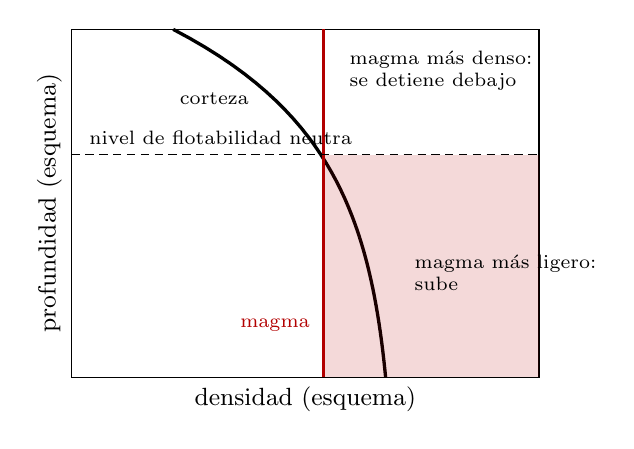
\begin{tikzpicture}[font=\scriptsize]
\begin{axis}[width=0.62\linewidth, height=6cm,
  xmin=0, xmax=1.15, ymin=0, ymax=1, y dir=reverse,
  xtick=\empty, ytick=\empty,
  xlabel={densidad (esquema)}, ylabel={profundidad (esquema)},
  label style={font=\small}, clip=false]
\addplot[very thick, black, domain=0:1, samples=40] ({0.25 + 0.55*(1 - exp(-3*x))}, {x});
\addplot[very thick, red!70!black] coordinates {(0.62,0) (0.62,1)};
\fill[red!70!black, opacity=0.15] (axis cs:0.62,0.36) rectangle (axis cs:1.15,1);
\draw[densely dashed] (axis cs:0,0.36) -- (axis cs:1.15,0.36);
\node[anchor=south west] at (axis cs:0.02,0.36) {nivel de flotabilidad neutra};
\node[anchor=east, black] at (axis cs:0.46,0.20) {corteza};
\node[anchor=east, red!70!black] at (axis cs:0.61,0.85) {magma};
\node[anchor=west, align=left] at (axis cs:0.82,0.70) {magma más ligero:\\sube};
\node[anchor=west, align=left] at (axis cs:0.66,0.12) {magma más denso:\\se detiene debajo};
\end{axis}
\end{tikzpicture}
\par\smallskip{\small El \omterm{def:b2:magma-emplacement:ascent}{nivel de flotabilidad neutra} (esquema). La densidad de
la corteza aumenta con la profundidad, por compactación de los sedimentos y por el paso a
rocas más densas; un \omterm{def:b2:magma-emplacement:magma}{magma} de densidad fija sube mientras es más ligero que su
entorno (sombreado) y se extiende donde las dos densidades se igualan.}
\end{omfigure}

Un \omterm{def:b2:magma-emplacement:bodies}{plutón} debe hacerse sitio. Puede levantar su techo, como hace un \omterm{def:b2:magma-emplacement:bodies}{lacolito};
puede apartar sus paredes donde son blandas; puede llenar el espacio abierto por
fallas; y puede desprender su techo, bloque a bloque. Durante mucho tiempo se imaginaron los grandes plutones
como enormes depósitos de \omterm{def:b2:magma-emplacement:magma}{magma} emplazados de una sola vez. La datación ha cambiado esa
imagen. Los circones de la Suite Intrusiva de Tuolumne, un \omterm{def:b2:magma-emplacement:bodies}{batolito} granítico de
California, muestran que se emplazó entre \num{95} y \qty{85}{Ma}, con lo más antiguo
en los bordes y lo más joven en el centro, y una sola de sus unidades durante más
de \qty{3}{Myr}, entre \qty{92.8}{Ma} y \qty{88.8}{Ma}. Un único cuerpo de
\omterm{def:b2:magma-emplacement:magma}{magma} de \qty{5}{km} de espesor y \qty{20}{km} de anchura emplazado a \qty{15}{km} de profundidad se
habría enfriado por debajo de \qty{750}{\celsius}, donde está cristalizado a medias, en
unos \num{500000}~años. Estos plutones deben de haberse ensamblado de forma incremental,
a partir de muchas intrusiones menores, como láminas y \omterm{def:b2:magma-emplacement:bodies}{diques}, a lo largo de millones de años
(\cref{exo:b2:magma-emplacement:11}).
% ledger: glazner04:tuolumne

\begin{omfigure}
\centering
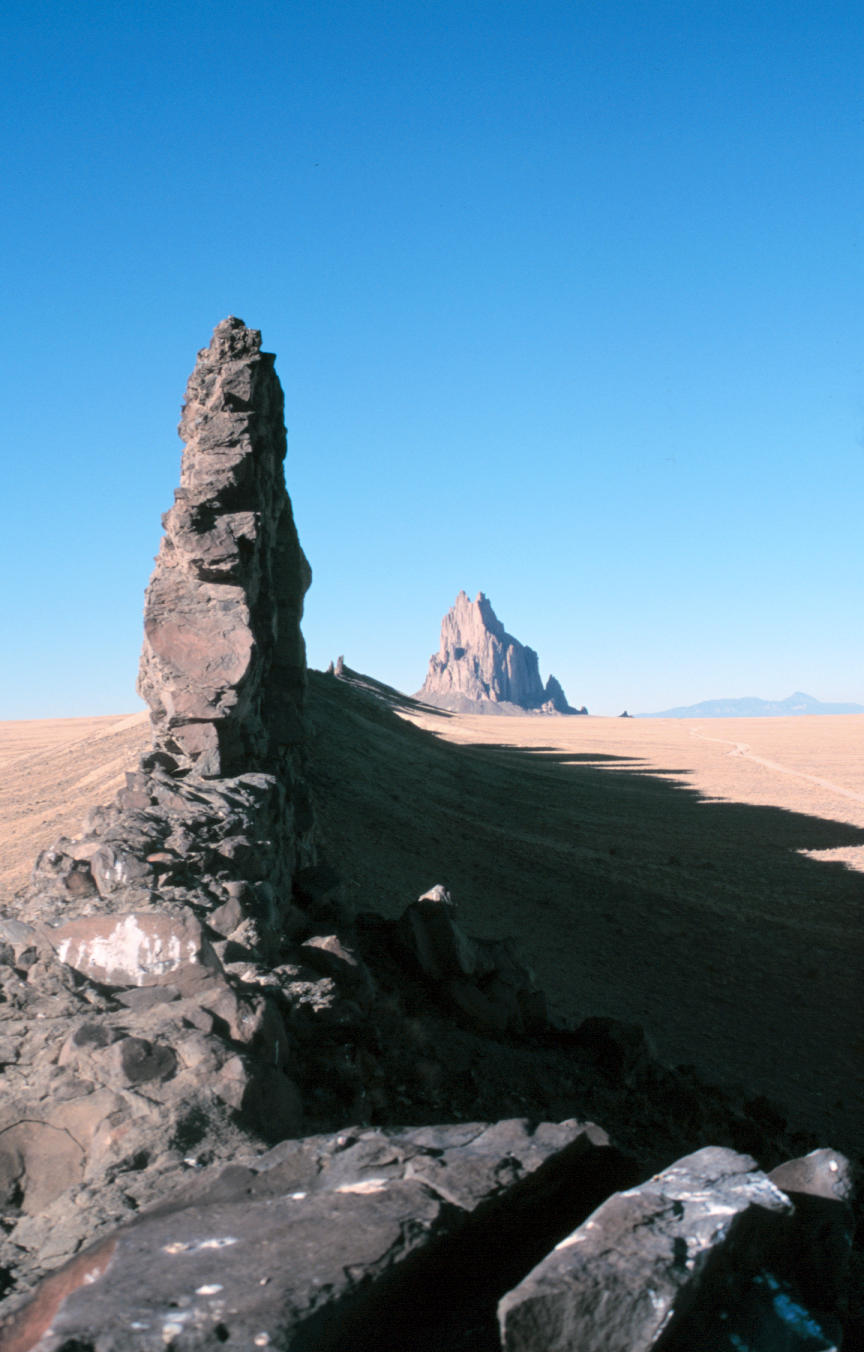
\includegraphics[width=0.3\linewidth]{images/book4/b2-shiprock-dyke.jpg}
\par\smallskip{\small Un \omterm{def:b2:magma-emplacement:bodies}{dique} cerca de Shiprock, en el campo volcánico navajo
(Nuevo México): la roca del \omterm{def:b2:magma-emplacement:bodies}{dique} resistió la erosión mejor que la arenisca y la lutita
que cortaba, y hoy se alza como un muro; al fondo, el cuello volcánico del que
irradian varios \omterm{def:b2:magma-emplacement:bodies}{diques} como este. Fotografía: Dexter Perkins (CC0).}
\end{omfigure}

\section{Enfriamiento y metamorfismo de contacto}

Una intrusión pierde su calor por conducción hacia su roca encajante. El modelo más sencillo
trata la intrusión y su encajante como un único medio conductor de
difusividad uniforme $\kappa$: en el instante cero una lámina de espesor $b$ está a la temperatura
de intrusión $T_m$ y el encajante a $T_0$. La solución de la ecuación del calor, con
$x$ medida desde el centro de la lámina, es
\[
T(x,t) = T_0 + \frac{T_m - T_0}{2}\left[\operatorname{erf}\frac{b/2 - x}{2\sqrt{\kappa t}}
+ \operatorname{erf}\frac{b/2 + x}{2\sqrt{\kappa t}}\right].
\]
La figura siguiente la muestra para un \omterm{def:b2:magma-emplacement:bodies}{filón capa} de \qty{100}{m} de espesor.
% ledger: delaney86b4:properties

\begin{proposition}[Temperatura de contacto]\label{prop:b2:magma-emplacement:contact}
En este modelo, mientras $\sqrt{\kappa t}$ sea pequeño frente a $b$, la
temperatura en el contacto de la intrusión se mantiene en la media $(T_m + T_0)/2$ de
las temperaturas de la intrusión y del encajante.
\end{proposition}

\begin{proof}
En el contacto $x = b/2$ la primera función error es $\operatorname{erf}0 = 0$ y
la segunda es $\operatorname{erf}(b/(2\sqrt{\kappa t}))$, que es cercana a $1$ mientras
$b \gg 2\sqrt{\kappa t}$. Entonces $T = T_0 + (T_m - T_0)/2$.
\end{proof}

Un \omterm{def:b2:magma-emplacement:bodies}{dique} basáltico a \qty{1150}{\celsius} en rocas a \qty{50}{\celsius} calienta así
su contacto a \qty{600}{\celsius}. El calor de cristalización, típicamente de
\qtyrange{700}{1000}{MJ/m^3}, mantiene el \omterm{def:b2:magma-emplacement:magma}{magma} caliente más tiempo y eleva este valor:
con \qty{900}{MJ/m^3} liberados entre \num{1150} y \qty{950}{\celsius} el mismo
modelo da \qty{690}{\celsius}, mientras que las conductividades dependientes de la temperatura y los encajantes
húmedos rebajan ambas estimaciones entre 50 y \qty{75}{\celsius}.
% ledger: delaney86b4:dike, delaney86b4:properties

\begin{omfigure}
\centering
\begin{tikzpicture}
\begin{axis}[omrecord, width=0.86\linewidth, height=6cm,
  xmin=-200, xmax=200, ymin=0, ymax=1200,
  xlabel={distancia al centro del filón capa (\unit{m})},
  ylabel={temperatura (\unit{\celsius})},
  legend pos=north east, legend style={font=\scriptsize},
  tick label style={font=\scriptsize}, label style={font=\small}]
\fill[gray!15] (axis cs:-50,0) rectangle (axis cs:50,1200);
\addplot[very thick, red!80!black] table[x=x_m, y=t1] {figdata/out/bachelor-2-magma-sill.dat};
\addlegendentry{1 año}
\addplot[very thick, orange!90!black] table[x=x_m, y=t2] {figdata/out/bachelor-2-magma-sill.dat};
\addlegendentry{10 años}
\addplot[very thick, blue!60!black] table[x=x_m, y=t3] {figdata/out/bachelor-2-magma-sill.dat};
\addlegendentry{50 años}
\addplot[very thick, black] table[x=x_m, y=t4] {figdata/out/bachelor-2-magma-sill.dat};
\addlegendentry{200 años}
\draw[densely dashed, gray] (axis cs:-200,625) -- (axis cs:200,625);
\node[font=\scriptsize, gray!40!black, anchor=south west] at (axis cs:-198,625) {$(T_m + T_0)/2$};
\node[font=\scriptsize, anchor=south] at (axis cs:0,20) {filón capa};
\end{axis}
\end{tikzpicture}
\par\smallskip{\small Enfriamiento conductivo de un \omterm{def:b2:magma-emplacement:bodies}{filón capa} de \qty{100}{m} de espesor (sombreado),
intruido a \qty{1150}{\celsius} en una roca a \qty{100}{\celsius}, con
$\kappa = \qty{0.7e-6}{m^2/s}$ y sin calor latente. El contacto se mantiene cerca de
\qty{625}{\celsius} durante décadas mientras el calor se extiende por el encajante; al cabo de dos
siglos el \omterm{def:b2:magma-emplacement:bodies}{filón capa} y su entorno forman una sola zona templada amplia.}
\end{omfigure}
% ledger: delaney86b4:properties

La escala de tiempo del enfriamiento es el tiempo que el calor necesita para difundirse a través de la
intrusión, del orden de $(b/2)^2/\kappa$: unos \num{16} días para un \omterm{def:b2:magma-emplacement:bodies}{dique}
de \qty{2}{m} de anchura, un siglo para un \omterm{def:b2:magma-emplacement:bodies}{filón capa} de \qty{100}{m} de espesor, cien mil años
para un \omterm{def:b2:magma-emplacement:bodies}{plutón} de unos pocos kilómetros. El calor latente la alarga, y también la
necesidad de solidificar el \omterm{def:b2:magma-emplacement:magma}{magma} y no solo enfriarlo.

\begin{proposition}[Solidificación de una intrusión]\label{prop:b2:magma-emplacement:stefan}
Llene un \omterm{def:b2:magma-emplacement:magma}{magma} a su temperatura de solidificación $T_m$, con calor latente $L$ por unidad de
volumen, el espacio $y > 0$ junto a una roca encajante a $T_0$ que ocupa $y < 0$, ambos
de capacidad calorífica $\rho c$ por unidad de volumen y difusividad $\kappa$. El
frente de solidificación avanza como $y_s = 2\lambda\sqrt{\kappa t}$, donde $\lambda$
es la raíz de
\[
\frac{L\sqrt\pi}{\rho c\,(T_m - T_0)} = \frac{e^{-\lambda^2}}{\lambda\,(1 + \operatorname{erf}\lambda)},
\]
y el contacto se mantiene a $T_0 + (T_m - T_0)/(1 + \operatorname{erf}\lambda)$. Un \omterm{def:b2:magma-emplacement:bodies}{filón capa}
de espesor $b$, que se solidifica desde ambas paredes, es sólido al cabo de
$t = b^2/(16\lambda^2\kappa)$.
\end{proposition}

\begin{proof}
El \omterm{def:b2:magma-emplacement:magma}{magma} por delante del frente permanece a $T_m$, de modo que el calor solo fluye en el sólido
y en el encajante, donde se ensaya $T = T_0 + (T_m - T_0)(1 + \operatorname{erf}\xi)/(1 +
\operatorname{erf}\lambda)$ con $\xi = y/(2\sqrt{\kappa t})$. Toda función de $\xi$
de la forma $\alpha + \beta\operatorname{erf}\xi$ resuelve la ecuación del calor; esta
tiende a $T_0$ lejos en el encajante ($\xi \to -\infty$) y vale $T_m$ en el frente
$\xi = \lambda$. En $y = 0$ da la temperatura de contacto enunciada. En el frente,
el calor latente liberado por el sólido que avanza, $L\,dy_s/dt = L\lambda\sqrt{\kappa/t}$
por unidad de área y de tiempo, debe evacuarse por conducción, $k\,\partial T/\partial y = k(T_m -
T_0)\,e^{-\lambda^2}/[(1 + \operatorname{erf}\lambda)\sqrt{\pi\kappa t}]$. Igualando ambos
y usando $k = \rho c\kappa$ se obtiene la ecuación de $\lambda$. Cada pared del
\omterm{def:b2:magma-emplacement:bodies}{filón capa} hace crecer su propio frente, de forma independiente mientras el núcleo permanece a $T_m$; los dos
frentes se encuentran cuando $2\lambda\sqrt{\kappa t} = b/2$.
\end{proof}

Con el calor latente de un basalto y un encajante a unos \qty{100}{\celsius},
$\lambda$ vale cerca de $0.65$: un \omterm{def:b2:magma-emplacement:bodies}{filón capa} de \qty{100}{m} de espesor se solidifica en unos
setenta años, y su contacto se mantiene cerca de \qty{740}{\celsius} en lugar de
\qty{625}{\celsius} mientras lo hace. El problema de fin de semana desarrolla este caso.
Como el tiempo crece como el cuadrado del espesor, un \omterm{def:b2:magma-emplacement:bodies}{filón capa} diez veces más grueso
tarda cien veces más.

\begin{definition}[La aureola de contacto y sus rocas]\label{def:b2:magma-emplacement:aureole}
Un \emph{borde de enfriamiento rápido}\index{borde de enfriamiento rápido} es el borde de grano fino o vítreo de una
intrusión, donde el \omterm{def:b2:magma-emplacement:magma}{magma} se enfrió deprisa contra una roca encajante más fría. Una
\emph{aureola de contacto}\index{aureola de contacto} es la zona de roca encajante que rodea una
intrusión y que fue metamorfizada por su calor. La \emph{corneana}\index{corneana} es la
roca dura, de grano fino y no foliada en que se convierten las lutitas y las rocas volcánicas en
una aureola de contacto. El \emph{skarn}\index{skarn} es la roca que se forma donde los fluidos
magmáticos calientes reaccionan con un encajante carbonatado y depositan silicatos de
calcio, hierro y magnesio como el granate y el piroxeno, a menudo con magnetita y sulfuros metálicos.
\end{definition}
% ledger: earle:intrusive-bodies, earle:skarn

Las \omterm{def:b2:magma-emplacement:aureole}{aureolas de contacto} van de unos pocos centímetros alrededor de los \omterm{def:b2:magma-emplacement:bodies}{diques} y filones capa pequeños a
varias decenas de metros alrededor de un stock grande, y el metamorfismo de contacto abarca
desde unos \qty{300}{\celsius} hasta más de \qty{800}{\celsius}. Una lutita se convierte en una
\omterm{def:b2:magma-emplacement:aureole}{corneana}, una caliza en un mármol, una arenisca en una cuarcita. Un \omterm{def:b2:magma-emplacement:magma}{magma} emplazado a gran profundidad
en rocas que ya están calientes apenas forma aureola: la anchura depende del
tamaño y de la temperatura de la intrusión y de la temperatura de su encajante, como
predice el modelo de enfriamiento (\cref{exo:b2:magma-emplacement:12}). Los minerales que crecen en una aureola,
y lo que dicen de la temperatura, corresponden al \cref{ch:b2:metamorphic-facies};
los metales que concentran los \omterm{def:b2:magma-emplacement:aureole}{skarns}, al \cref{ch:b2:ore-deposits}.
% ledger: earle:skarn

\begin{inthefield}[Leer los contactos de un dique]
\begin{minipage}[t]{0.6\linewidth}\vspace{0pt}
Donde aflora un \omterm{def:b2:magma-emplacement:bodies}{dique}, un geólogo sigue primero sus contactos con la roca
encajante. Un borde de grano más fino o más vítreo que el centro del \omterm{def:b2:magma-emplacement:bodies}{dique} indica
que el \omterm{def:b2:magma-emplacement:magma}{magma} se enfrió bruscamente contra una roca fría; un \omterm{def:b2:magma-emplacement:bodies}{dique} de \qty{25}{cm} de anchura estudiado
en la costa de la Columbia Británica tiene \omterm{def:b2:magma-emplacement:aureole}{bordes de enfriamiento rápido} de \qty{2}{cm} de espesor. A continuación se examina la roca
encajante junto al contacto en busca de cocción: un cambio de color, un endurecimiento,
minerales nuevos que se desvanecen al alejarse del \omterm{def:b2:magma-emplacement:bodies}{dique}. La anchura de la zona cocida y del
\omterm{def:b2:magma-emplacement:aureole}{borde de enfriamiento rápido}, medida frente a la anchura del \omterm{def:b2:magma-emplacement:bodies}{dique}, indica lo caliente que estaba
el encajante cuando llegó el \omterm{def:b2:magma-emplacement:bodies}{dique}; un \omterm{def:b2:magma-emplacement:bodies}{dique} sin \omterm{def:b2:magma-emplacement:aureole}{borde de enfriamiento rápido} ni
aureola se intruyó en rocas que ya estaban calientes. Se toman muestras a través del
\omterm{def:b2:magma-emplacement:bodies}{dique}, del borde al centro, para la geoquímica de su fundido y para el
tamaño de sus cristales.
\end{minipage}\hfill
\begin{minipage}[t]{0.36\linewidth}\vspace{0pt}
\centering
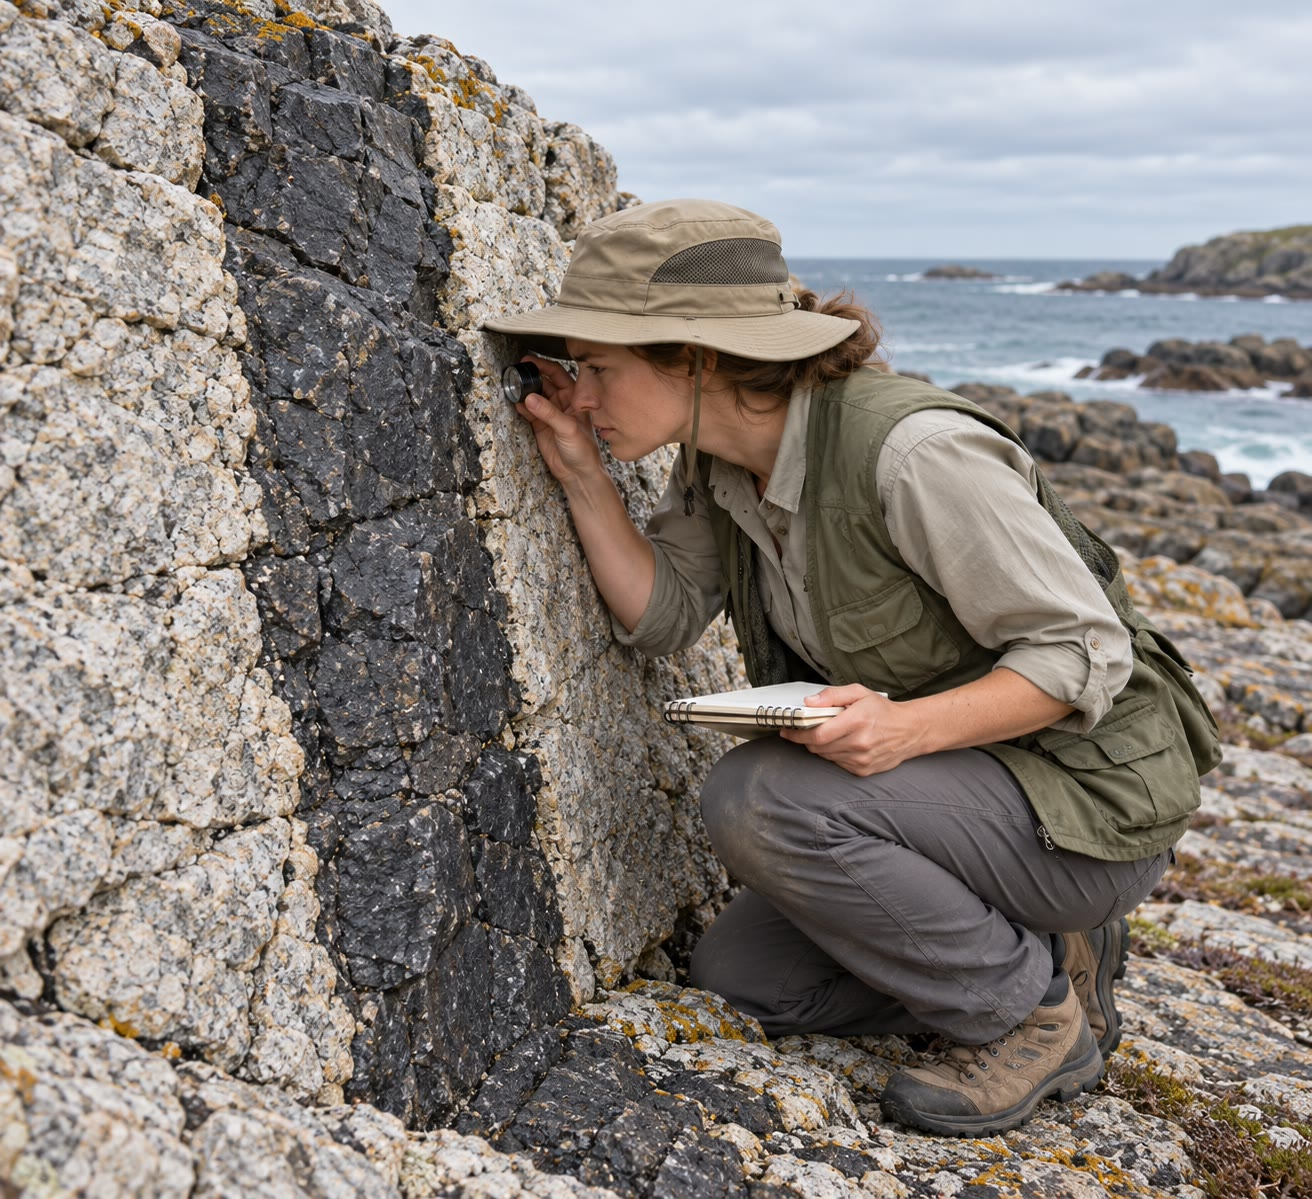
\includegraphics[width=\linewidth]{images/book4/ai/b2-dyke-contact.jpg}
\par\smallskip{\scriptsize Un geólogo examina el contacto de un \omterm{def:b2:magma-emplacement:bodies}{dique} oscuro con
una roca encajante clara (ilustración generada por IA).}
\end{minipage}
\end{inthefield}
% ledger: earle:intrusive-bodies

\section{Ejercicios}

\begin{exercise}[$\star$]\label{exo:b2:magma-emplacement:1}
Para los fundidos graníticos hidratados, una ecuación ajustada a medidas da
$\log_{10}\eta = [-3.545 + 0.833\ln w] + [9601 - 2368\ln w]/\{T - [195.7 + 32.25\ln
w]\}$, con $\eta$ en \unit{Pa.s}, $w$ el contenido en agua en porcentaje en masa y $T$
en kelvin. Calcúlese $\log_{10}\eta$ a \qty{800}{\celsius} para $w = 1$ y $w = 4$,
y el factor en que los tres por ciento de agua adicionales reducen la viscosidad.
\end{exercise}
% ledger: hd96:model

\begin{exercise}[$\star$]\label{exo:b2:magma-emplacement:2}
Con la ley de la raíz cuadrada, $s = 0.44$ para una riolita y $s = 0.34$ para un basalto
(por ciento en masa por $\sqrt{\unit{MPa}}$), calcúlense la presión de saturación de una
riolita con un \qty{6}{\percent} de agua y de un basalto con un \qty{0.5}{\percent},
y las profundidades correspondientes en una corteza de densidad \qty{2600}{kg/m^3}
($g = \qty{9.81}{m/s^2}$).
\end{exercise}

\begin{exercise}[$\star$]\label{exo:b2:magma-emplacement:3}
Calcúlese la temperatura de contacto de un \omterm{def:b2:magma-emplacement:bodies}{dique} basáltico a \qty{1150}{\celsius}
intruido en rocas a \qty{50}{\celsius}, y luego en rocas a
\qty{400}{\celsius}. ¿Cuál de los dos \omterm{def:b2:magma-emplacement:bodies}{diques} tendrá el \omterm{def:b2:magma-emplacement:aureole}{borde de enfriamiento rápido} más ancho?
\end{exercise}

\begin{exercise}[$\star$]\label{exo:b2:magma-emplacement:4}
Nómbrese cada cuerpo. (a) Una lámina de dolerita de \qty{30}{m} de espesor situada entre dos capas
de arenisca a lo largo de \qty{20}{km}. (b) Una lámina vertical de basalto de \qty{2}{m} de anchura
que corta calizas horizontales. (c) Un granito que aflora en \qty{2000}{km^2},
formado por una docena de unidades de edades distintas. (d) Una lente de pórfido de \qty{1}{km} de diámetro,
plana en su base, sobre la cual las capas están arqueadas. (e) Una lámina horizontal
de basalto en un granito.
\end{exercise}

\begin{exercise}[$\star\star$]\label{exo:b2:magma-emplacement:5}
Un fundido basáltico tiene $\eta_{\ell} = \qty{100}{Pa.s}$. Con la relación de Einstein--Roscoe
($R = 1.35$), calcúlese la viscosidad del \omterm{def:b2:magma-emplacement:magma}{magma} con un
\qty{5}{\percent}, un \qty{20}{\percent}, un \qty{40}{\percent} y un \qty{60}{\percent} de
cristales, y compárese la primera con la fórmula diluida de Einstein. ¿Con qué fracción
de cristales predice la relación el bloqueo?
\end{exercise}

\begin{exercise}[$\star\star$]\label{exo:b2:magma-emplacement:6}
Un \omterm{def:b2:magma-emplacement:magma}{magma} con una densidad \qty{300}{kg/m^3} menor que la de sus paredes sube por un \omterm{def:b2:magma-emplacement:bodies}{dique}.
(a) Para un basalto ($\eta = \qty{100}{Pa.s}$, $\rho = \qty{2700}{kg/m^3}$) en un \omterm{def:b2:magma-emplacement:bodies}{dique}
de \qty{1}{m} de anchura, calcúlense la velocidad media, el caudal por metro de \omterm{def:b2:magma-emplacement:bodies}{dique}, el
número de Reynolds y el tiempo para subir \qty{10}{km}. (b) El mismo tiempo para una riolita de
\qty{e6}{Pa.s} en un \omterm{def:b2:magma-emplacement:bodies}{dique} de \qty{1}{m} de anchura, y luego de \qty{10}{m}. (c) Un \omterm{def:b2:magma-emplacement:bodies}{dique}
de \qty{1}{m} de anchura pierde su calor en un tiempo del orden de $(w/2)^2/\kappa$, con $\kappa =
\qty{1e-6}{m^2/s}$: ¿cuál de los tres ascensos puede tener éxito?
\end{exercise}

\begin{exercise}[$\star\star$]\label{exo:b2:magma-emplacement:7}
Un \omterm{def:b2:magma-emplacement:magma}{magma} de densidad \qty{2400}{kg/m^3} a \qty{900}{\celsius} libera el
\qty{1}{\percent} de su masa como vapor de agua. Tratando el vapor como un gas ideal
($R = \qty{8.314}{J/(mol.K)}$, \qty{18.015}{g/mol}), calcúlese la fracción de volumen de
gas en el \omterm{def:b2:magma-emplacement:magma}{magma} a \qty{100}{MPa}, \qty{10}{MPa} y \qty{0.1}{MPa}. ¿Cuál de los
tres valores es el menos fiable, y por qué?
\end{exercise}

\begin{exercise}[$\star\star$]\label{exo:b2:magma-emplacement:8}
En una cuenca, la densidad de las rocas aumenta con la profundidad $z$ según $\rho(z) =
2300 + 60\,z$ (\unit{kg/m^3}, $z$ en \unit{km}) hasta \qty{10}{km}. (a) ¿Dónde está
el \omterm{def:b2:magma-emplacement:ascent}{nivel de flotabilidad neutra} de un fundido basáltico de \qty{2650}{kg/m^3}? (b) El
modelo de densidad de este capítulo muestra que un uno por ciento de agua disuelta reduce
la densidad de un fundido basáltico en unos \qty{70}{kg/m^3}. ¿Dónde se detiene un fundido con
un uno por ciento más de agua? (c) ¿Cuál es la fuerza de flotabilidad por metro cúbico
del fundido seco \qty{2}{km} por debajo de su \omterm{def:b2:magma-emplacement:ascent}{nivel de flotabilidad neutra}?
\end{exercise}

\begin{exercise}[$\star\star$]\label{exo:b2:magma-emplacement:9}
Supóngase que un \omterm{def:b2:magma-emplacement:ascent}{diapiro} granítico de radio \qty{1}{km} y déficit de densidad
\qty{300}{kg/m^3} sube a través de una corteza inferior de viscosidad \qty{e19}{Pa.s}. Calcúlense
su velocidad de Stokes (esfera rígida) en milímetros por año y el tiempo para subir
\qty{10}{km}. Compárese con la escala de tiempo $a^2/\kappa$ de su enfriamiento, con $\kappa
= \qty{1e-6}{m^2/s}$. ¿Qué se concluye?
\end{exercise}

\begin{exercise}[$\star\star\star$]\label{exo:b2:magma-emplacement:10}
El agua se disuelve en un fundido a la vez como moléculas, $x_m = K_1 f$, y como grupos
hidroxilo, $x_{\mathrm{OH}}^2 = K_2 x_m$ (con el oxígeno del fundido en gran exceso), de modo
que el agua disuelta total es $x = x_m + x_{\mathrm{OH}}/2$. (a) Exprésese $x$ en
función de $f$ y demuéstrese que se comporta como $\sqrt f$ para $f$ baja y como $f$ para
$f$ alta. (b) ¿A qué fugacidad son igual de abundantes las dos formas del agua? (c)
Con $K_1 = \qty{1e-4}{MPa^{-1}}$ y $K_2 = 0.2$, calcúlense esa fugacidad y la
proporción de agua disuelta como hidroxilo a \qty{100}{MPa}.
\end{exercise}

\begin{exercise}[$\star\star\star$]\label{exo:b2:magma-emplacement:11}
Un \omterm{def:b2:magma-emplacement:bodies}{plutón} granítico de \qty{1000}{km^3} se ensambla a lo largo de \qty{4}{Myr}. (a) Calcúlese
su aporte medio de \omterm{def:b2:magma-emplacement:magma}{magma} en \unit{km^3} por año y en \unit{m^3} por segundo. (b) Lo alimenta
un único \omterm{def:b2:magma-emplacement:bodies}{dique} de \qty{1}{km} de longitud y \qty{2}{m} de anchura, con una velocidad media de
\qty{0.8}{m/s}: ¿cuánto tardaría el \omterm{def:b2:magma-emplacement:bodies}{dique} en aportar todo el
\omterm{def:b2:magma-emplacement:bodies}{plutón}? ¿Qué fracción de los \qty{4}{Myr} es eso? (c) Si el \omterm{def:b2:magma-emplacement:bodies}{plutón} está formado por
láminas de \qty{20}{m} de espesor y \qty{10}{km} por \qty{10}{km} de extensión, ¿cuántas láminas
hacen falta, y cuánto tiempo separa de media dos de ellas? (d) Con
$\lambda = 0.65$ y $\kappa = \qty{0.7e-6}{m^2/s}$, ¿cuánto tarda una lámina en
solidificarse? ¿Es el \omterm{def:b2:magma-emplacement:bodies}{plutón} alguna vez un único gran cuerpo de \omterm{def:b2:magma-emplacement:magma}{magma}?
\end{exercise}

\begin{exercise}[$\star\star\star$]\label{exo:b2:magma-emplacement:12}
Lejos de un \omterm{def:b2:magma-emplacement:bodies}{dique} delgado de anchura $b$ (a distancias $x \gg b$), su calor actúa como una
fuente plana instantánea: $T - T_0 = (T_m - T_0)\,b\,e^{-x^2/(4\kappa
t)}/\sqrt{4\pi\kappa t}$. (a) Demuéstrese que a la distancia $x$ la temperatura es máxima en
$t^* = x^2/(2\kappa)$, y que este aumento máximo es $\Delta T_{\max} = (T_m -
T_0)\,b/(x\sqrt{2\pi e})$. (b) Para un \omterm{def:b2:magma-emplacement:bodies}{dique} de \qty{2}{m} de anchura con $T_m - T_0 =
\qty{1100}{K}$, ¿a qué distancia se calienta la roca como mucho \qty{100}{K}, y
cuándo ($\kappa = \qty{0.7e-6}{m^2/s}$)? (c) ¿Por qué son tan estrechas las aureolas de los
\omterm{def:b2:magma-emplacement:bodies}{diques} delgados?
\end{exercise}

\section{Problema: el filón capa bajo la meseta}

\begin{problem}[{Problema de fin de semana --- seguir un magma basáltico desde su dique
alimentador hasta un filón capa, su agua, y el tiempo que el filón capa tarda en solidificarse}]
\label{pb:b2:magma-emplacement:1}
Bajo una meseta imaginaria, unos sedimentos (lutita y arenisca) de densidad media
\qty{2450}{kg/m^3} descansan a \qty{3.0}{km} de profundidad sobre un basamento cristalino de
densidad \qty{2800}{kg/m^3}. Un \omterm{def:b2:magma-emplacement:magma}{magma} basáltico subió desde \qty{15}{km} por un \omterm{def:b2:magma-emplacement:bodies}{dique}
de \qty{2.0}{m} de anchura y se extendió a lo largo de la base de los sedimentos como un \omterm{def:b2:magma-emplacement:bodies}{filón capa} de dolerita
de \qty{100}{m} de espesor. Datos: temperatura de intrusión \qty{1150}{\celsius}; ley de viscosidad
del fundido $\log_{10}\eta = -4.55 + 5510/(T - 611)$ ($T$ en kelvin); densidad
del fundido con su agua \qty{2710}{kg/m^3}; un \qty{20}{\percent} de cristales en volumen
(Einstein--Roscoe, $R = 1.35$); agua disuelta \qty{0.40}{\percent}, solubilidad
$s = 0.34$ por ciento por $\sqrt{\unit{MPa}}$; temperatura del encajante en el \omterm{def:b2:magma-emplacement:bodies}{filón capa}
\qty{100}{\celsius}; $\kappa = \qty{0.7e-6}{m^2/s}$, $\rho c = \qty{2.5}{MJ/(m^3.K)}$,
calor latente \qty{900}{MJ/m^3}, considerándose que el \omterm{def:b2:magma-emplacement:magma}{magma} se solidifica a su
temperatura de intrusión; $g = \qty{9.81}{m/s^2}$; un año son \qty{3.156e7}{s}.

\medskip\noindent\textbf{Parte I --- El magma.}
\begin{enumerate}
\item Calcúlense $\log_{10}\eta$ y $\eta$ del fundido a \qty{1150}{\celsius}
(\qty{1423}{K}).
\item Lo mismo a \qty{1100}{\celsius}. ¿En qué factor cambia la viscosidad en
estos \qty{50}{K}?
\item Calcúlese la viscosidad del \omterm{def:b2:magma-emplacement:magma}{magma} con sus cristales a
\qty{1150}{\celsius}.
\item ¿Con qué fracción de cristales haría la relación de Einstein--Roscoe que el
\omterm{def:b2:magma-emplacement:magma}{magma} se bloqueara? Compárese con la estimación de campo del final del flujo en masa.
\item Calcúlese la diferencia de densidad entre el \omterm{def:b2:magma-emplacement:magma}{magma} y el basamento, y
entre el \omterm{def:b2:magma-emplacement:magma}{magma} y los sedimentos.
\item Calcúlese la presión litostática al nivel del \omterm{def:b2:magma-emplacement:bodies}{filón capa}.
\end{enumerate}

\noindent\textbf{Parte II --- Subiendo por el dique.}
\begin{enumerate}[resume]
\item Calcúlese el gradiente de presión por flotabilidad $\Delta\rho\,g$ que impulsa el \omterm{def:b2:magma-emplacement:magma}{magma}
a través del basamento.
\item Calcúlese la velocidad media del \omterm{def:b2:magma-emplacement:magma}{magma} en el \omterm{def:b2:magma-emplacement:bodies}{dique}.
\item Calcúlense el caudal por metro de \omterm{def:b2:magma-emplacement:bodies}{dique} y el caudal total si el \omterm{def:b2:magma-emplacement:bodies}{dique} tiene
\qty{1.0}{km} de longitud.
\item Calcúlese el número de Reynolds del flujo. ¿Es laminar?
\item ¿Cuánto tarda el \omterm{def:b2:magma-emplacement:magma}{magma} en subir de \qty{15}{km} a \qty{3.0}{km}?
\item Compárese con la escala de tiempo $(w/2)^2/\kappa$ en la que el \omterm{def:b2:magma-emplacement:bodies}{dique} pierde su
calor. ¿Puede mantenerse abierto?
\item Explíquese por qué el \omterm{def:b2:magma-emplacement:magma}{magma} se detuvo a \qty{3.0}{km} y se extendió lateralmente, usando
el vocabulario del capítulo.
\end{enumerate}

\noindent\textbf{Parte III --- El agua.}
\begin{enumerate}[resume]
\item Calcúlese la presión de saturación del agua del fundido, y la profundidad en los
sedimentos a la que se alcanza.
\item ¿Cuánta agua podría contener el fundido al nivel del \omterm{def:b2:magma-emplacement:bodies}{filón capa}? ¿Exsuelve agua el \omterm{def:b2:magma-emplacement:magma}{magma}
del \omterm{def:b2:magma-emplacement:bodies}{filón capa}?
\item Las vesículas del \omterm{def:b2:magma-emplacement:aureole}{borde de enfriamiento rápido} del \omterm{def:b2:magma-emplacement:bodies}{filón capa} contienen sobre todo CO$_2$. Explíquese.
\item Si todo el \qty{0.40}{\percent} de agua saliera en la superficie, a
\qty{1150}{\celsius} y \qty{0.1}{MPa}, ¿qué fracción de volumen del \omterm{def:b2:magma-emplacement:magma}{magma} ocuparía
el vapor (gas ideal)?
\end{enumerate}

\noindent\textbf{Parte IV --- Enfriamiento y solidificación.}
\begin{enumerate}[resume]
\item Sin tener en cuenta el calor latente, calcúlese la temperatura de contacto del \omterm{def:b2:magma-emplacement:bodies}{filón capa}.
\item Sin tener en cuenta el calor latente, calcúlese la temperatura \qty{10}{m} por encima del contacto
superior \num{10}~años después de la intrusión.
\item Con el mismo modelo, calcúlese la temperatura en el centro del \omterm{def:b2:magma-emplacement:bodies}{filón capa} al cabo de
\num{10}~años y de \num{50}~años.
\item Con el mismo modelo, \qty{80}{m} por encima del contacto superior, calcúlese la temperatura al cabo de
\num{300}, \num{363} y \num{420} años. ¿Llega alguna vez la roca de ese punto a
\qty{300}{\celsius}?
\item Calcúlese $L\sqrt\pi/(\rho c\,(T_m - T_0))$ para el \omterm{def:b2:magma-emplacement:bodies}{filón capa}.
\item Evalúese $e^{-\lambda^2}/(\lambda(1 + \operatorname{erf}\lambda))$ para $\lambda = 0.64$,
$0.65$ y $0.66$ ($\operatorname{erf}0.64 = 0.6346$, $\operatorname{erf}0.65 = 0.6420$,
$\operatorname{erf}0.66 = 0.6494$), y dese $\lambda$ con dos decimales.
\item Con calor latente, calcúlese la temperatura de contacto mientras el \omterm{def:b2:magma-emplacement:bodies}{filón capa}
se solidifica. ¿Por qué es más alta que en la pregunta 18?
\item Calcúlese la escala de tiempo $(b/2)^2/\kappa$ en años.
\item Calcúlese el tiempo que tarda el \omterm{def:b2:magma-emplacement:bodies}{filón capa} en solidificarse, en años, el número clave de
este problema, y explíquese por qué es más corto que la escala de tiempo de la
pregunta anterior aunque haya que evacuar el calor latente.
\end{enumerate}
\end{problem}
% ledger: grd08:model, kolz22:einstein-roscoe, glazner04:tuolumne, moore98:h2o, lowenstern01:co2, delaney86b4:properties
